\section{Horseshoe shrinkage model}
\label{sec:regression}

\subsection{Motivation}
The logit model of Section \ref{sec:logit} was fit on the small set of
covariates suggested by the brief, taking their usefulness for granted. That is
a reasonable baseline, but it leaves open the central question of the analysis:
among \emph{all} the available predictors, in particular the fourteen
service-quality ratings that were set aside earlier, which ones actually carry
signal for customer satisfaction, and which are redundant? Rather than answering
this by hand, adding and removing covariates and guessing at their relevance, we
prefer a principled, automatic mechanism. We therefore fit a Bayesian logistic
regression on the \emph{full} set of covariates under a \textbf{horseshoe}
shrinkage prior \cite{bl_book}, which is designed to pull the coefficients of
noise predictors strongly towards zero while leaving genuine signals almost
untouched. This lets the data, rather than our prior guesses, single out the
meaningful covariates.

\subsection{Model specification}
We include all $21$ standardised predictors: the $14$ service-quality items
plus \texttt{age}, \texttt{flight\_distance}, the two cabin-class dummies
(\textit{Eco Plus}, \textit{Business}), $\log(1+\texttt{dep\_delay})$,
\textit{Personal Travel} and \textit{disloyal Customer} - and, as in Section
\ref{sec:logit}, the mid-flight delay is kept outside the design matrix with its
own coefficient $\beta_{\text{arr}}$. The likelihood is again Bernoulli with a
logit link:
\begin{equation}
    y_i \mid p_i \sim \text{Bernoulli}(p_i),
    \qquad
    \text{logit}(p_i) = \beta_0 + x_i^\top \beta
        + \beta_{\text{arr}}\,\texttt{arr\_delay}_i .
    \label{eq:hs_model}
\end{equation}

The horseshoe prior replaces the common vague Gaussian of Section
\ref{sec:logit} with a scale-mixture of normals: each coefficient gets its own
\emph{local} scale $\lambda_j$, and all local scales share a single
\emph{global} scale $\tau$,
\begin{equation}
    \beta_j \mid \lambda_j, \tau \sim \mathcal{N}(0, \lambda_j^2 \tau^2),
    \qquad
    \lambda_j \sim \mathcal{C}^+(0,1),
    \qquad
    \tau \sim \mathcal{C}^+(0,1),
    \label{eq:hs_prior}
\end{equation}
where $\mathcal{C}^+(0,1)$ denotes the standard half-Cauchy distribution. The
global scale $\tau$ pulls \emph{all} coefficients towards zero, enforcing overall
sparsity, while the heavy Cauchy tails of the local scales $\lambda_j$ let
individual coefficients escape that shrinkage when the data demand it - this is
precisely the ``a few large, most near zero'' behaviour that makes the prior
suited to feature selection. The arrival-delay coefficient
$\beta_{\text{arr}}$ is given its own local scale $\lambda_{\text{arr}}$ under
the \emph{same} global $\tau$, so that it competes for signal on an equal footing
with the other $21$ predictors. Following the JAGS notes, each half-Cauchy is
implemented as a Student-$t$ with one degree of freedom truncated to the positive
reals, \texttt{dt(0, 1, 1)\,T(0, )}. The intercept keeps a diffuse Gaussian
prior, $\beta_0 \sim \mathcal{N}(0, 100)$ (i.e. \texttt{dnorm(0, 0.01)}), and is
deliberately left out of the shrinkage so that the baseline log-odds is not
penalised.

A convenient by-product of the mixture form is the \emph{shrinkage weight}
\begin{equation}
    \kappa_j = \frac{1}{1 + \lambda_j^2},
    \qquad \kappa_j \in (0,1),
    \label{eq:kappa}
\end{equation}
which measures how much coefficient $j$ is pulled towards zero: $\kappa_j$ near
$0$ marks a preserved \emph{signal} (essentially unshrunk), whereas $\kappa_j$
near $1$ marks a coefficient shrunk towards \emph{noise}. We use the posterior
distribution of the $\kappa_j$ as our covariate-relevance summary.

\subsection{MCMC setup and convergence}
Because of the heavy-tailed half-Cauchy hyperpriors, the horseshoe posterior
mixes more slowly than the vague-prior model of Section \ref{sec:logit}, and it
is computationally heavier ($22$ coefficients, $22$ local scales and one global
scale, against the $9$ parameters of Section \ref{sec:logit}). We therefore
budget a longer sampling run and thinning from the outset; the settings, reported
in Table \ref{tab:hs_mcmc_settings}, are deliberately modest given the
single-core environment and could be extended on a larger machine.

Convergence was assessed separately for the two blocks of parameters, the
regression coefficients $\{\beta_j, \beta_0, \beta_{\text{arr}}\}$ and the scale
parameters $\{\lambda_j, \lambda_{\text{arr}}, \tau\}$, since the latter are the
harder to sample. For each block we inspected the Gelman--Rubin potential scale
reduction factors, the effective sample sizes, and the trace and autocorrelation
plots. The coefficients mix well and show scale-reduction factors close to $1$;
the scale parameters, and $\tau$ in particular, mix more slowly and show higher
autocorrelation, as expected for a horseshoe, but reach effective sample sizes
adequate for the summaries we report. Figures \ref{fig:hs_trace_beta} and
\ref{fig:hs_trace_lambda} show a representative trace plot for each block. The
complete diagnostic material - all trace and autocorrelation plots for both the
$\beta$ and the $\lambda$ parameters, together with the full Gelman--Rubin and
effective-sample-size tables - is collected in Appendix
\ref{app:mcmc_horseshoe}.

\subsection{Posterior results}
Figure \ref{fig:hs_posterior} shows the marginal posterior densities of the
coefficients: most concentrate tightly around zero, with only a handful clearly
displaced, which is the visual signature of the shrinkage at work. The relevance
ranking is made explicit in Figure \ref{fig:hs_shrinkage}, which plots the
posterior distribution of the shrinkage weights $\kappa_j$ of
Eq.~\eqref{eq:kappa}: predictors on the ``signal'' side ($\kappa_j$ small) are
the ones the model retains, while those pushed to $\kappa_j \to 1$ are treated as
redundant. Figure \ref{fig:hs_forest} reports the same information on the
coefficient scale, as a forest plot of the posterior means and $95\%$ credible
intervals of the $\beta_j$, colouring in the covariates identified as signal
($\kappa_j < 0.5$).

\begin{figure}[htbp]
\centering
\begin{subfigure}[t]{0.48\linewidth}
  \centering
  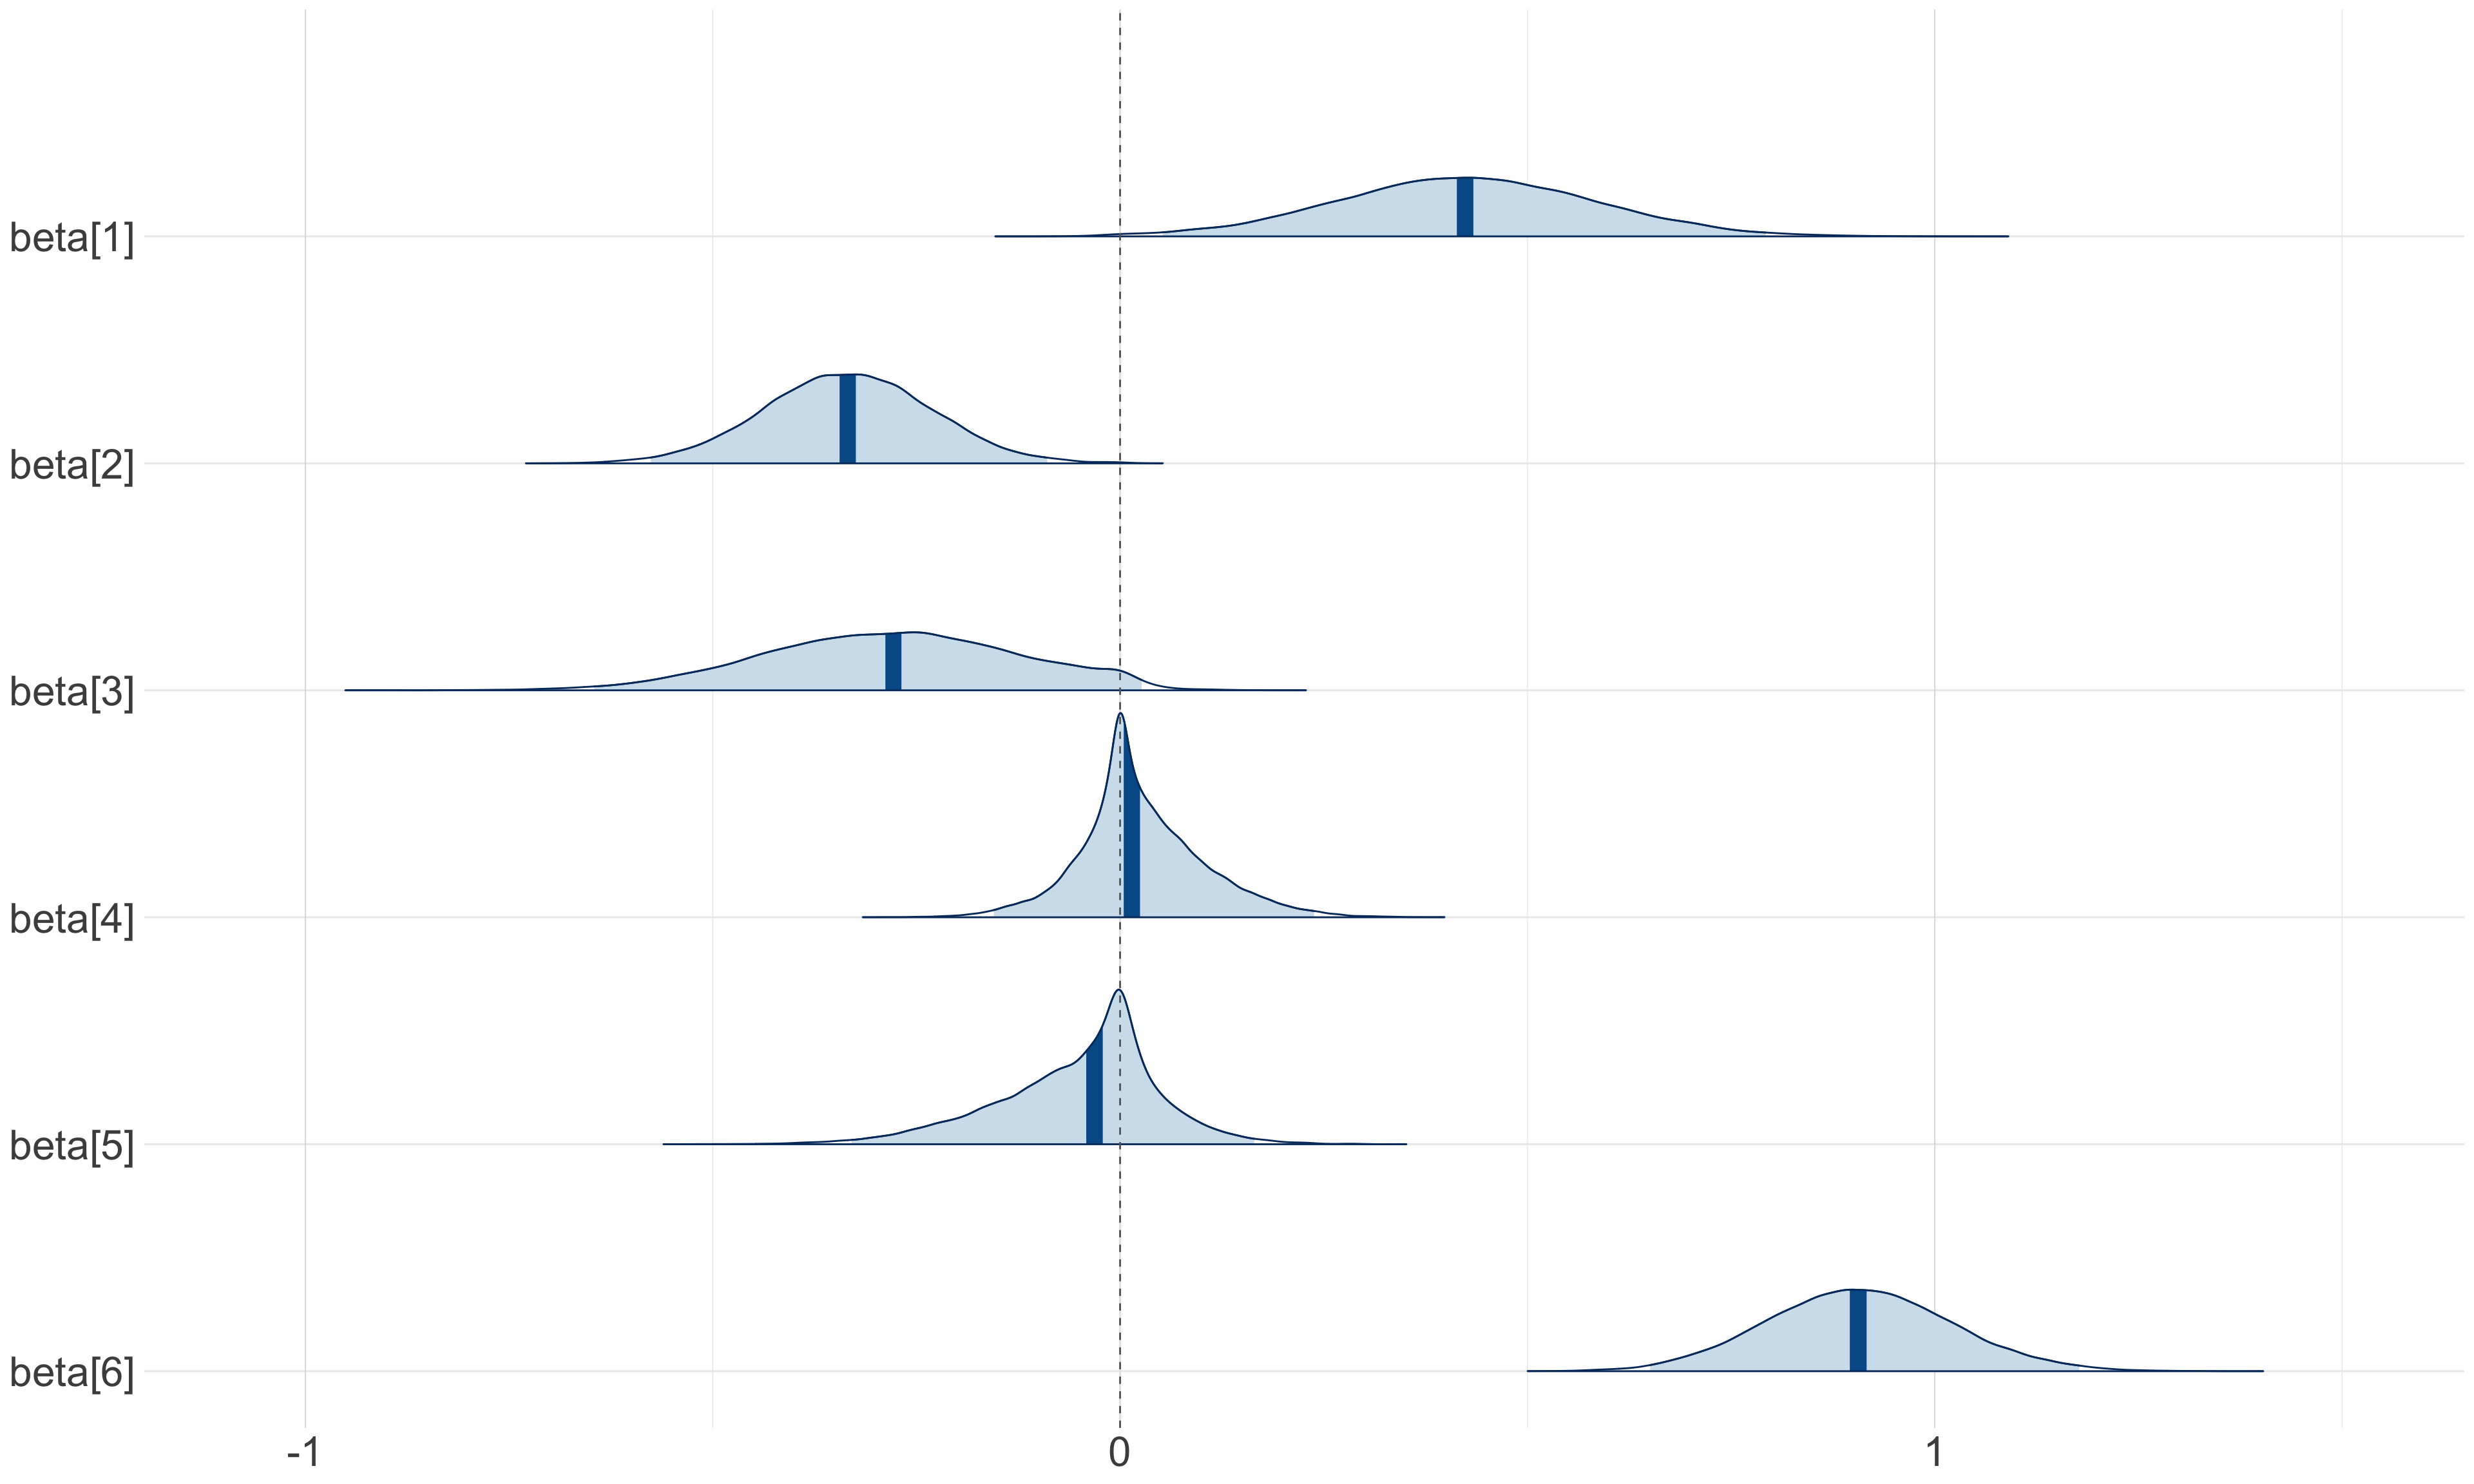
\includegraphics[width=\linewidth]{img/horseshoe_model/post1.png}
  \caption{Marginal posterior densities of the coefficients under the horseshoe
           prior ($98\%$ intervals). Most coefficients are shrunk tightly around
           zero; only a few escape.}
  \label{fig:hs_posterior}
\end{subfigure}\hfill
\begin{subfigure}[t]{0.48\linewidth}
  \centering
  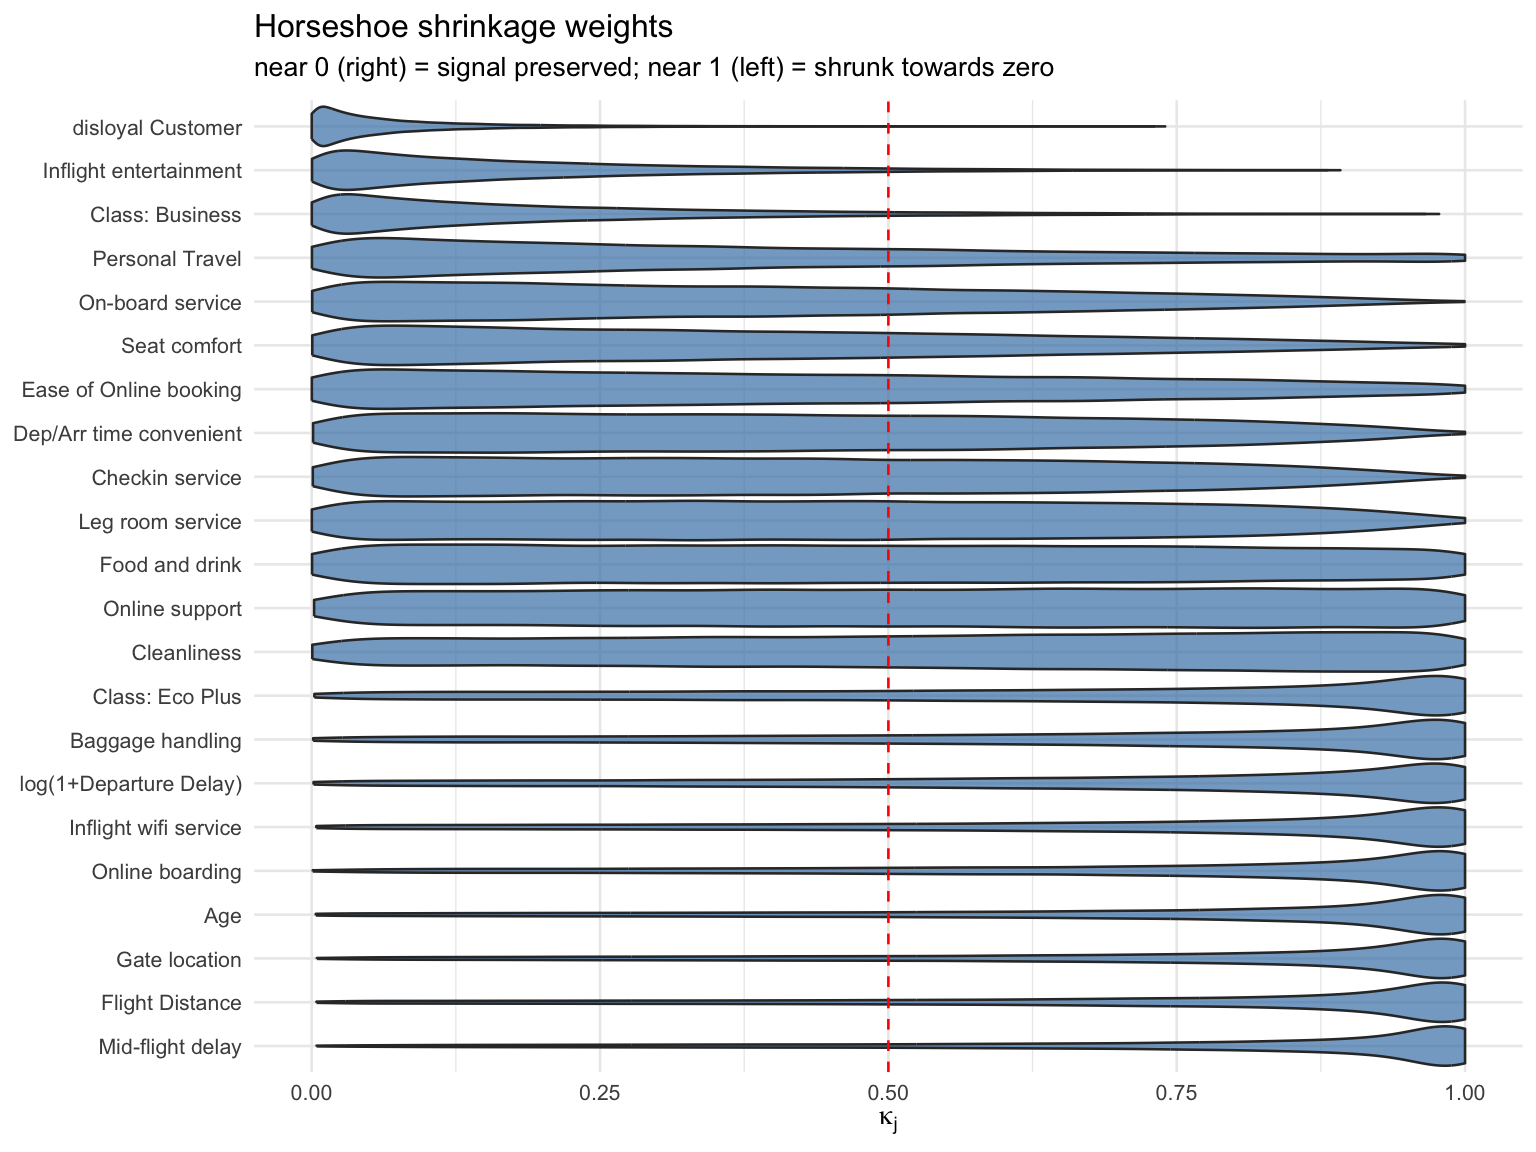
\includegraphics[width=\linewidth]{img/horseshoe_model/shrinkage_beta.png}
  \caption{Posterior distribution of the horseshoe shrinkage weights $\kappa_j$
           for each predictor. Near $0$ (right) the signal is preserved; near $1$
           (left) the coefficient is shrunk towards zero. The dashed line marks
           $\kappa_j = 0.5$.}
  \label{fig:hs_shrinkage}
\end{subfigure}
\end{figure}

\begin{figure}[htbp]
  \centering
  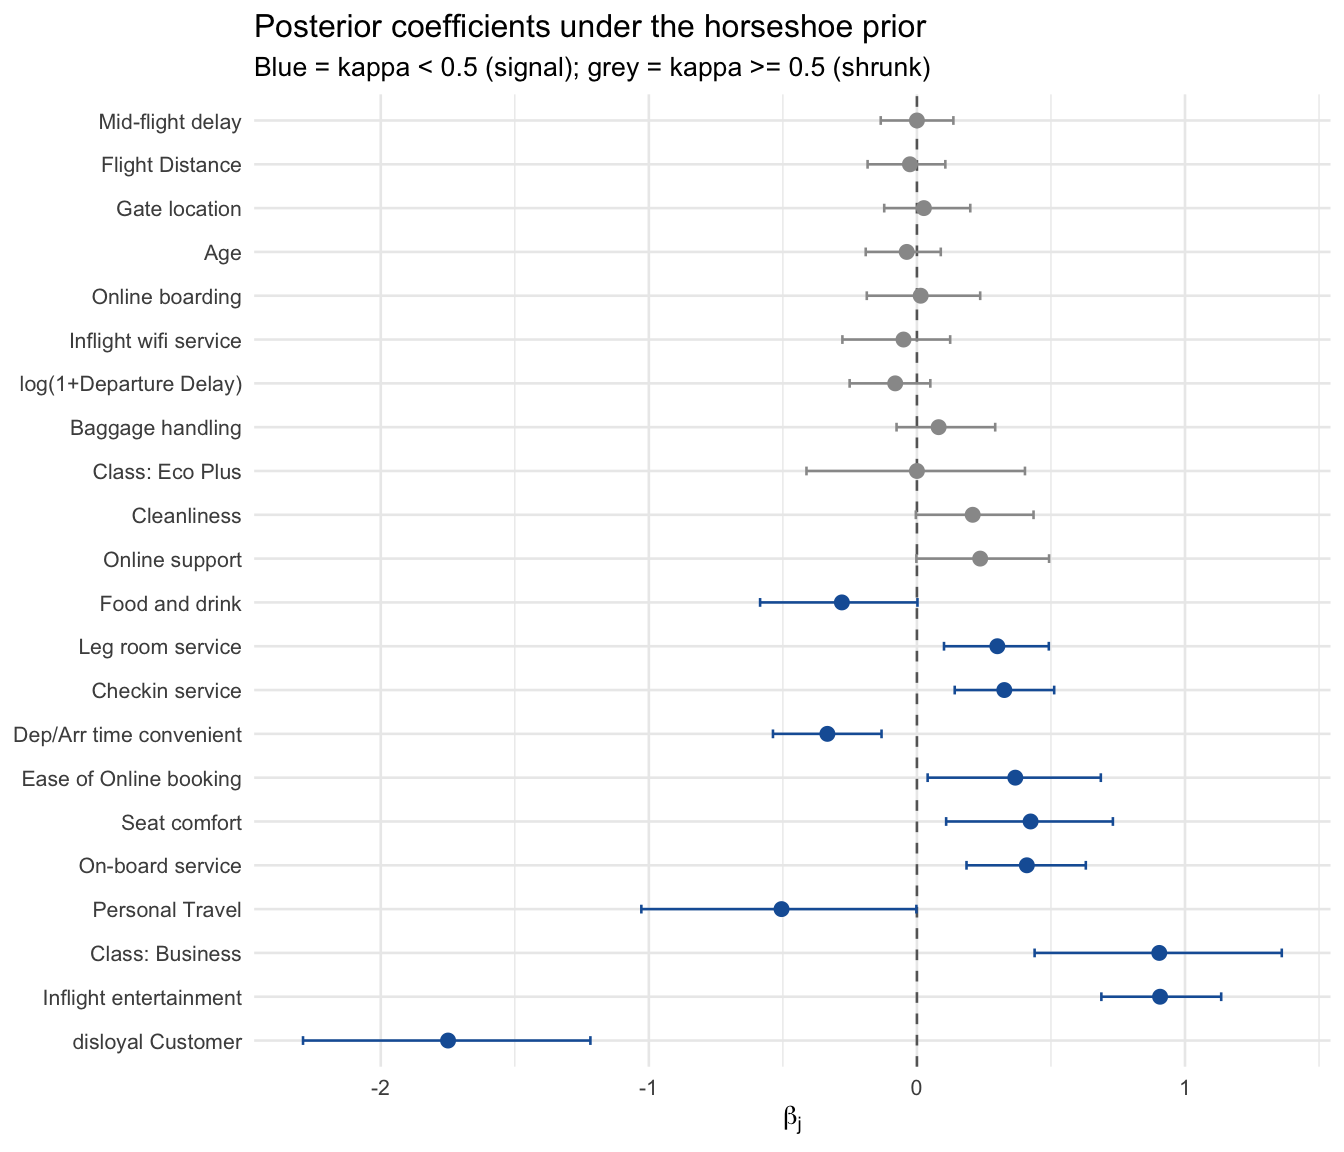
\includegraphics[width=0.75\linewidth]{img/horseshoe_model/beta_forest.png}
  \caption{Posterior coefficients $\beta_j$ under the horseshoe prior (means and
           $95\%$ credible intervals). Blue marks the covariates identified as
           signal ($\kappa_j < 0.5$), grey the shrunk ones.}
  \label{fig:hs_forest}
\end{figure}

\subsection{Conclusions}
The horseshoe cleanly separates the informative predictors from the redundant
ones, and several of its findings sharpen - and in one case reverse - the
picture from Sections \ref{sec:data_expl} and \ref{sec:logit}.

\paragraph{The booking / connectivity cluster visibly competes.}
Among the four mutually correlated ``booking / connectivity'' items identified in
the exploratory analysis (Section \ref{sec:data_expl}), the prior does not treat
them symmetrically: \textit{Ease of Online booking} and \textit{Online support}
are preserved noticeably more than \textit{Online boarding} and
\textit{Inflight wifi service} - the latter being the single most shrunk item in
the whole model. This is exactly the mechanism the horseshoe was chosen for: when
several correlated items carry overlapping information, the prior lets two of them
represent the signal and treats the other two as largely redundant, instead of
forcing us to pick one by hand.

\paragraph{Business class shrinks once service quality is in the model.}
In Section \ref{sec:logit}, \textit{Business} class alone carried a large,
confident odds ratio (about $4$). Here, with all $14$ service ratings included,
its coefficient shrinks markedly and its credible interval crosses zero. The
natural reading is \emph{mediation}, not disappearance: Business passengers are
more satisfied largely \emph{because} they enjoy better seat comfort,
entertainment and service, so in Section \ref{sec:logit} the \textit{Class}
dummy was partly standing in for those ratings simply because they were not yet
in the model.

\paragraph{Personal Travel gets stronger, not weaker.}
Section \ref{sec:logit} found the type-of-travel effect nearly explained away by
\textit{Class}. Under the horseshoe, once the service ratings control for the
\emph{quality} of the trip experience, \textit{Personal Travel} re-emerges as one
of the strongest and most confidently negative effects in the model, with a
credible interval lying entirely below zero. The two findings are not
contradictory: they show that the earlier attenuation was specifically about
\textit{Class} soaking up part of the travel-type signal, not about travel type
being unimportant.

\paragraph{A cautionary sign on time convenience.}
More tentatively, \textit{Departure/Arrival time convenient} has a
\emph{negative} posterior mean with a credible interval excluding zero - higher
ratings associated with \emph{lower} satisfaction, which is counter-intuitive.
Recall from Section \ref{sec:data_expl} that this item has one of the largest
shares of structural zeros and sits in its own correlated cluster with
\textit{Seat comfort}, \textit{Food and drink} and \textit{Gate location}; its
zeros plausibly encode ``not applicable'' rather than genuine dissatisfaction.
We therefore read this coefficient as a candidate symptom of that ambiguity
rather than a reliable substantive finding, and revisit it directly in the
structural-zero robustness check of Section \ref{sec:robustness}.

\paragraph{Loyalty dominates throughout.}
Finally, \textit{disloyal Customer} remains, by a wide margin, the single
strongest and most confidently preserved effect in the entire model - consistent
across the exploratory analysis and both models of Sections \ref{sec:logit} and
\ref{sec:regression}, regardless of how many other covariates are present.

% -----------------------------------------------------------------------------
% NOTE: the .Rmd conclusions quote exact posterior figures via inline `r ...`
% code (specific kappa_j values, the Business/Personal-Travel/time-convenient
% posterior means and 95% credible-interval endpoints). Those numbers come from
% the knitted run and were not available when this draft was written, so they
% are described qualitatively above. Fill in the precise values from the
% kappa_tbl of notebook 03 (03_horseshoe_summary.rds) where desired.
% -----------------------------------------------------------------------------
